\chapter{Тележка и меандр}
\label{ch:chap4}
\section{Условие задачи}

Рассмотрим систему, состоящую из тележки и генератора задающего сигнала:
$$
  \begin{cases}
    \dot{x} = Ax + Bu, \tab x(0)= \begin{bmatrix} 0 & 0 \end{bmatrix}^T, \\
    \dot{w_g} = \text{Г}w_g, \tab w_g(0) = \begin{bmatrix} 0 & 1 & 0 & 1 &  0 & 1 & 0 & 1\end{bmatrix}^T \\
    z = C_Zx + D_z w_g
  \end{cases}
$$ и выполним следующие шаги:

\begin{itemize}
    \item Синтезировать математическую модель «тележки», приняв в качестве выхода 
    линейную координату $y(t) = x_1(t)$.
    \item Принять задающий сигнал $g(t)$ меандром с произвольной амплитудой и периодом (выбрать самостоятельно).
    \item Разложить сигнал $g(t)$ в ряд Фурье и задаться конечным числом гармоник $m$ для использования конечной суммы ряда в качестве приближенного сигнала $\bar{g}(t)$.
    \item Сформировать генератор, способный порождать выбранные гармоники
    компоненты $\bar{g}(t)$. Необходимый порядок генератора определить самостоятельно.
    \item Задаться виртуальным выходом $z(t)$ в форме и задать матрицы $(C_Z, D_Z)$ такими, 
    чтобы при выполнении целевого условия было справедливо:
    
    $$
     \bar{g}(t) = D_Z w_g(t), \tab \lim_{t\to +\infty} |\bar{g}(t) - y(t)| = 0
    $$

    \item Прокомментировать, какую задачу вы решаете таким образом.
    
    \item  Синтезировать следящий регулятор, обеспечивающий выполнение целевого
    условия. Привести выкладки процедуры синтеза и полученные матрицы $K_1$ и $K_2$.
    \item Выполнить моделирование и построить графики формируемого регулятором управления $u(t)$, 
    вектора состояния замкнутой системы $x(t)$, задающего сигнала $g(t)$, приближенного задающего сигнала $\bar{g}(t)$ и
    выхода $y(t)$.
    \item Проанализировать полученные результаты и сделать выводы о достоинствах и недостатках такого регулятора.


\end{itemize}

Начальные данные:

$$
  A = \begin{bmatrix}
    0 & 1 \\ 0 & 0
\end{bmatrix}, \tab B = \begin{bmatrix}
  0 \\
  1 
\end{bmatrix}, \tab C = \begin{bmatrix}
  1 \\ 0
\end{bmatrix}^T, \tab D = 0, 
$$


В качестве задающего сигнала $g(t)$ \href{https://ru.wikipedia.org/wiki/%D0%9C%D0%B5%D0%B0%D0%BD%D0%B4%D1%80_(%D1%80%D0%B0%D0%B4%D0%B8%D0%BE%D1%82%D0%B5%D1%85%D0%BD%D0%B8%D0%BA%D0%B0)?useskin=vector}{выберем меандр с единичной амплитудой}, период $w\pi$. 
Аппроксимируем этот сигнал с помощью частичной суммы ряда Фурье, $m=4$:
$$
    \bar{g}(t) = \frac{4}{\pi} sin(t) + \frac{4}{\pi} sin(t) + \frac{4}{3\pi} sin(3t) + \frac{4}{5\pi} sin(5t) + \frac{4}{7\pi} sin(7t)
$$

Сформируем генератор, способный порождать нужные нам гармоники:
$$
\text{Г} = \begin{bmatrix}
    0 & 1 & 0 & 0 & 0 & 0 & 0 & 0 \\
    -1 & 0 & 0 & 0 & 0 & 0 & 0 & 0 \\
    0 & 0 & 0 & 3 & 0 & 0 & 0 & 0 \\
    0 & 0 & -3 & 0 & 0 & 0 & 0 & 0 \\
    0 & 0 & 0 & 0 & 0 & 5 & 0 & 0 \\
    0 & 0 & 0 & 0 & -5 & 0 & 0 & 0 \\
    0 & 0 & 0 & 0 & 0 & 0 & 0 & 7 \\
    0 & 0 & 0 & 0 & 0 & 0 & -7 & 0 \\
\end{bmatrix}
$$
Не трудно заметить, что его собственные числа формируют нужные нам гармоники:
$$
    \sigma(\text{Г}) = \{ \pm 1i, \pm 3i, \pm 5i, \pm 7i \}
$$

Для задачи слежения:
$$
\bar{g}(t) = D_Z w_g(t), \tab \lim_{t\to +\infty} |\bar{g}(t) - y(t)| = 0
$$
Поэтому выберем матрицы $(C_Z, D_Z)$ такими:
$$
C_Z = \begin{bmatrix}
     1 \\ 0
    \end{bmatrix}, \tab 
D_Z = \begin{bmatrix}
    \frac{4}{\pi} & 0 & \frac{4}{3\pi} & 0 & \frac{4}{5\pi} & 0 & \frac{4}{7\pi} & 0
\end{bmatrix}
$$

\section{Решение задания}

Синтезируем «feedback»-компоненту $K_1$ с помощью \text{LQR}-регулятора, функционал качества:
$$
  J = \int_0^{\infty} (x^TQx + u^TRu) dt
$$ 
$$
  Q = \begin{bmatrix}
    1 & 0 &  \\
    0 & 1 & 
  \end{bmatrix}, \quad R = \begin{bmatrix}
    1
  \end{bmatrix}
$$
Получаем матрицу $K_1$:
$$
  K_1 = \begin{bmatrix}
    -1 & -1.73 \\
\end{bmatrix}
$$

Синтезируем «feedforward»-компоненту $K_2$:
$$
  K_2 = \begin{bmatrix}
    0 & 2.21 & -3.4 & 2.21 & -6.11 & 2.21 & -8.73 & 2.21 \\
\end{bmatrix}
$$



\begin{figure}[ht]
  \centering
  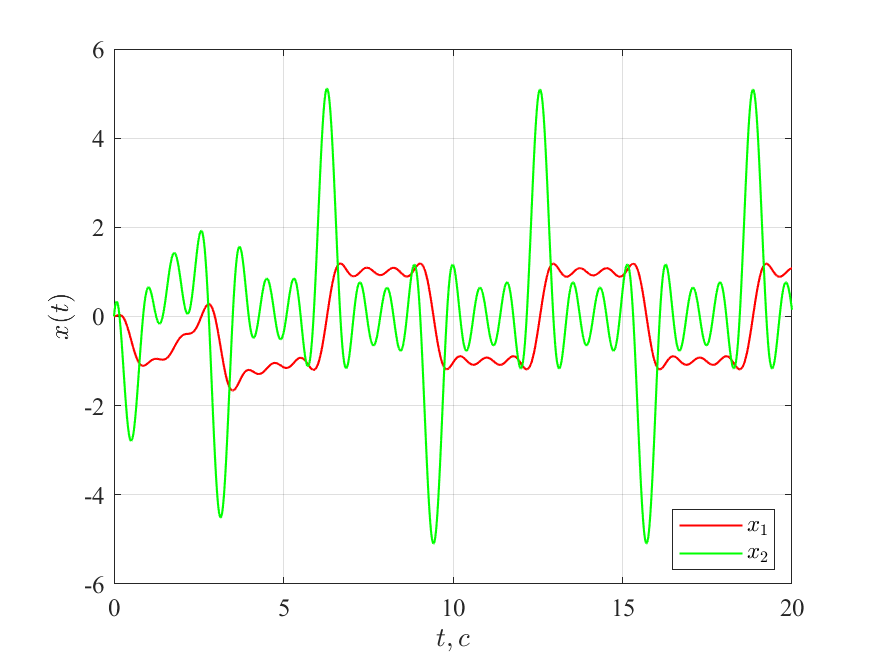
\includegraphics[width=0.8\textwidth]{x10.png}
  \caption{Моделирование - $x(t)$}
\end{figure}

\begin{figure}[ht]
  \centering
  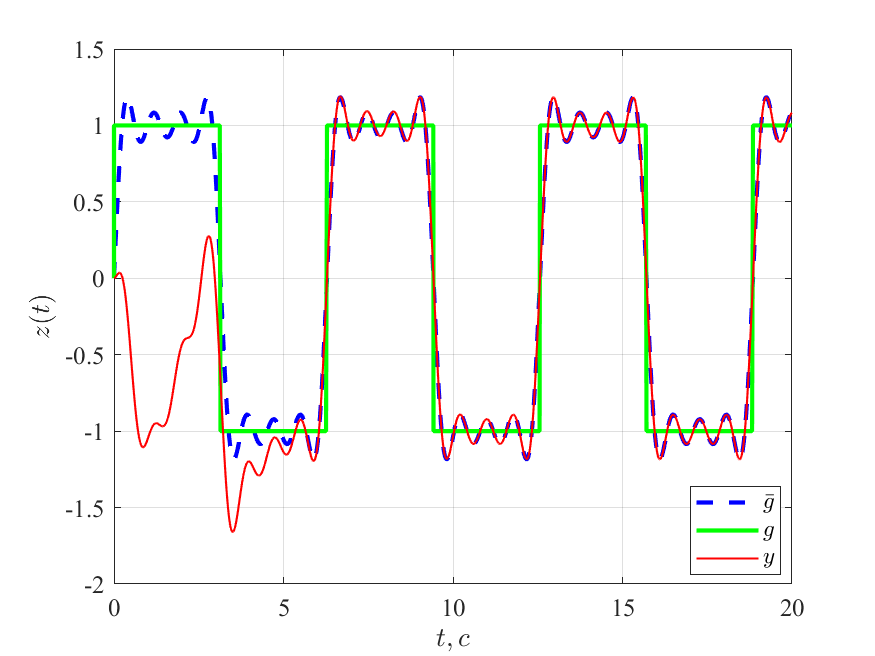
\includegraphics[width=0.8\textwidth]{y_compare.png}
  \caption{Моделирование - сравнение $y(t), g(t), \bar{g}(t)$}
\end{figure}

\begin{figure}[ht]
  \centering
  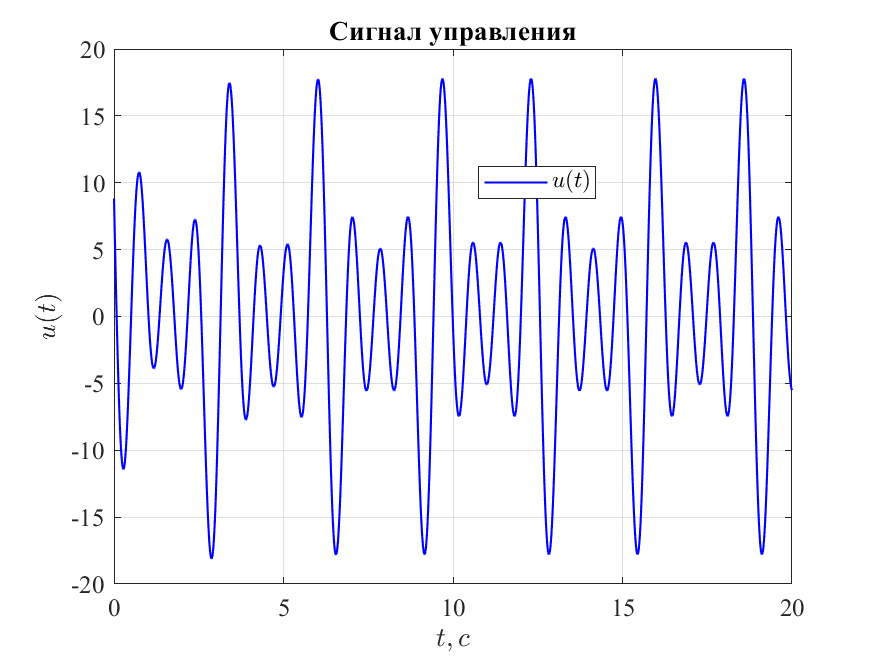
\includegraphics[width=0.8\textwidth]{u10.png}
  \caption{Моделирование - $u(t)$}
\end{figure}

\section{Выводы}

Наша система не способна следить за сигналами типа "меандр", но после аппроксимации такого генератора задающих сигналов посредством частичной суммы ряда Фурье, разложением на гармоники, 
мы уже смогли за ними проследить и решить задачу слежения относительного такого "приближённого" сигнала.

\endinput